%% LaTeX2e Template by Stephen Iota (https://stepheniota.com/)
%% last updated: May 2019
\documentclass[11pt]{article}
\usepackage[margin=2.5cm]{geometry}
\usepackage[utf8]{inputenc}
\usepackage{amsmath,amssymb,amsthm,physics}
\usepackage{mathtools} % for boxed answers in align environments
\usepackage{cancel}
\usepackage{graphicx}
%\usepackage[shortlabels]{enumitem} % change labels in enum/item environments
\usepackage[labelfont=bf,font=small]{caption}
\usepackage[dvipsnames]{xcolor}
%\usepackage[big]{titlesec} % [small,medium,big]
\usepackage{fancyhdr} %http://tug.ctan.org/tex-archive/macros/latex/contrib/fancyhdr/fancyhdr.pdf
%\usepackage[noadjust]{cite}
%\usepackage{lipsum}
\usepackage[
	colorlinks=true,
	citecolor=NavyBlue!90!black,
	linkcolor=green!50!black,
	urlcolor=RoyalBlue,
	hypertexnames=false]{hyperref}

%%%%%%%%%%%%%%%%%%%%%%%%%%%%%%%%
%% My commands & environments %%
%%%%%%%%%%%%%%%%%%%%%%%%%%%%%%%%
\newcommand{\email}[1]{\texttt{\href{mailto:#1}{#1}}}
\renewcommand{\d}[1]{\ensuremath{\operatorname{d}\!{#1}}}
%\newcommange{\ave}[1]{\ensuremath{\langle {#1} \rangle}}

%\newenvironment{question}[0]{
%\bigbreak
%\noindent
%}
\theoremstyle{definition}
\newtheorem{question}{Part}[section]
\newtheorem*{solution}{Solution}
%\newenvironment{solution}[0]{
%\bigbreak
%\noindent
%\textbf{Solution:}
%}

%%%%%%%%%%%%%%%%%%
%% Front Matter %%
%%%%%%%%%%%%%%%%%%
\pagestyle{fancy}
\fancyhead[L]{\footnotesize{\leftmark}}
\fancyhead[C]{}
\fancyhead[R]{\footnotesize{ IOTA \textbf{\thepage}}}
\fancyfoot[L,C,R]{}
\thispagestyle{plain} % no hf on first page
%\pagenumbering{gobble} % no page numbers
%\setcounter{section}{-1}
\graphicspath{{figures/}} % set directory for figures
\numberwithin{equation}{section}
\numberwithin{figure}{section}


%%%%%%%%%%%%%
%%% Title %%%
%%%%%%%%%%%%%
\begin{document}

\begin{center}
{\LARGE \textsc{Statistical Mechanics}: \textbf{Final Exam}}
\end{center}
\bigbreak

%%%%%%%%%%
%% INFO %%
%%%%%%%%%%
\begin{tabular}{rl}
\textsc{Name}:&		Stephen Iota (\email{siota001@ucr.edu})
\\
\textsc{Course}:&		Physics 133 (Spring 2019), Prof.~Kuhlman
\\
\textsc{Date}:&		\today
\end{tabular}
\bigbreak



%%%%%%%%%%%%%%
%% PROBLEMS %%
%%%%%%%%%%%%%%

\noindent
Sethna problems 2.1, 3.11, 5.2, 5.10, 7.3 and \textbf{An unlikely event}. Final answers are \boxed{\text{boxed}}.





%%%%%%%%%%%%%%%%%%%%%%%%%%%%%%%%%
%% RANDOM WALKS IN GRADE SPACE %%
%%%%%%%%%%%%%%%%%%%%%%%%%%%%%%%%%
\section{Random walks in grade space}
Consider a multiple-choice exam with ten questions of ten points each. Each problem on the exam is equally difficult. Students score a mean of $70$ on the exam. Assume all students are identical, and each question is answered at random with a probability of $0.7$ of being correct.

%%%%%%%%%%%%
%% PART A %%
%%%%%%%%%%%%
\begin{question}
\textbf{(a)}~What is the expected mean and standard deviation for the exam?
\end{question}

\begin{solution}
Let $p_+ = 0.7$ be the probability of a correct answer and $1 - p_+ = p_-$ be the probability of an incorrect answer; let $s \in \mathbb{S}$ be an exam score of a student in the set $\mathbb{S}$ of all possible student scores, and let $N$ be the number of questions on the exam. The mean score $\expval{s}$ is given by
\begin{equation}
\expval{s_N} = \sum_{n = 0}^N \binom{N}{n} \ (N-n)p_-\cdot(N-n)p_+\cdot10n \ \text{pts}
\end{equation}
and the rms score $\expval{s^2}$is
\begin{equation}
\expval{s_N^2} = \sum_{n = 0}^N \binom{N}{n} \ (N-n)p_-\cdot(N-n)p_+\cdot10n \ \text{pts}^2.
\end{equation}
Standard deviation $\sigma$ is related to the mean and rms by
\begin{equation}
\sigma = \sqrt{\expval{s^2} - \expval{s}^2}.
\end{equation}

First lets consider $N = 1$ questions on the exam. The mean, rms and std dev in this case are
\begin{align}
\expval{s_1} &= p_+(10 \ \text{pts}) = 7 \ \text{pts}
\\
\expval{s_1^2} &= p_+(10 \ \text{pts})^2 = 70 \ \text{pts}
\\
\sigma &= \sqrt{70 - 7^2} = \sqrt{21} \ \text{pts}
\end{align}
We can use the properties of random walks to see the evolution of these parameters as the number of questions on the exam $N$ increases. The mean score $\expval{s_N}$ will be $7N$ pts. The std dev scales by $\sqrt{N}$. This means that $\sigma_N = \sqrt{21N}$ pts.

For an exam of 10 questions, we find a mean of 10 pts and std dev of $\sqrt{210}$.
\begin{align}
\Aboxed{\expval{s_{10}} &= 10 \ \text{pts}}
\\
\Aboxed{\expval{s_{10}^2} &= \sqrt{210} \ \text{pts} \approx 14.5 \ \text{pts}}
\end{align}
\end{solution}


\newpage
%%%%%%%%%%%%
%% PART B %%
%%%%%%%%%%%%
\begin{question}
\textbf{(b)}~A typical exam with mean 70 might have an observed std dev of about 15. What physical interpretation do you make of the ratio of the random standard deviation and the observed one?
\end{question}

\begin{solution}
For a completely random model with 10 questions, the mean score is $\expval{s} = 50$ pts and the std dev is $\sigma_\text{random} = \sqrt{250}$.
\begin{equation}
\frac{\sigma}{\sigma_\text{random}} = \frac{\sqrt{210}}{\sqrt{250}} \approx \frac{14.5}{15.8} \approx 0.92
\end{equation}
Students in our model have a smaller spread of scores than in a completely random model. In our model, we made our students ``smarter.'' In a real exam setting, students rarely randomly guess on all questions. They have a higher probability of getting each question correct, which is why our model is slightly more accurate than the random model.
\end{solution}












%%%%%%%%%%%%%%%%%%%%%%%
%% Maxwell Relations %%
%%%%%%%%%%%%%%%%%%%%%%%
\newpage
\section{Maxwell relations}

Consider the microcanonical formula for the equilibrium energy $E(S,V,N)$ of some general system. One knows that the second derivatives of energy are symmetric; at fixed $N$, we get the same answer whichever order we take partial derivatives with respect to $S$ and $V$.

\begin{question}
\textbf{(a)} Use this to show the Maxwell relation
\begin{equation}
\pdv{T}{V}\eval_{S,N} = - \pdv{P}{S}\eval_{V,N}.\label{eq:2.0}
\end{equation}
Generate two other similar formul{\ae} by taking other second partial derivatives of $E$.
\end{question}

\begin{solution}
Consider the fundamental thermodynamic relation
\begin{equation}
\d{E} = T\d{S} - P\d{V} + \mu\d{N}.
\end{equation}
Keeping $N$ constant, take the following derivatives.
\begin{align}
\pdv{E}{V}\eval_{S,N} &= -P
\\
\pdv{S}\eval_{V,N} \pdv{E}{V}\eval_{S,N} &= - \pdv{P}{S}\eval_{V,N}\label{eq:2.1}
\end{align}
Since the second derivative of energy is symmetric, we can switch the order of integration in the second step.
\begin{align}
\pdv{V}\eval_{S,N} \pdv{E}{S}\eval_{V,N} &= \pdv{T}{S}\eval_{V,N}\label{eq:2.2}
\end{align}
From eq.~\eqref{eq:2.1} and \eqref{eq:2.2}, it follows that
\begin{equation}
\boxed{\pdv{T}{V}\eval_{S,N} = - \pdv{P}{S}\eval_{V,N}.}
\end{equation}

Using the same recipe, we can construct more Maxwell relations. Another relationship is given by taking partials of energy with respect to volume and number of particles.
\begin{align}
\pdv{E}{V}\eval_{S,N} &= -P
\\
\pdv{N}\eval_{S,V} \pdv{E}{V}\eval_{S,N} &= -\pdv{P}{N}\eval_{S,V}
\\
\pdv{V}\eval_{S,N} \pdv{E}{N}\eval_{S,V} &= \pdv{\mu}{N}\eval_{S,V}
\\
\Aboxed{\pdv{\mu}{V}\eval_{S,N} &= -\pdv{P}{N}\eval_{S,V}}
\end{align}
Another one by differentiating energy by entropy and number of particles.
\begin{align}
	\pdv{E}{S}\eval_{V,N} &= T
	\\
	\pdv{N}\eval_{S,V} \pdv{E}{S}\eval_{V,N} &= -\pdv{T}{N}\eval_{S,V}
	\\
	\pdv{S}\eval_{V,N} \pdv{E}{N}\eval_{S,V} &= \pdv{\mu}{S}\eval_{V,N}
	\\
	\Aboxed{\pdv{T}{N}\eval_{S,V} &= \pdv{\mu}{S}\eval_{V,N}}
\end{align}
\end{solution}

\begin{question}
\textbf{(b)}~Statistical mechanics check of the Maxwell relation. Using
\begin{equation}
S(E,V,N) = \frac{5}{2} Nk_B + Nk_B\log\Bigg[\frac{V}{Nh^3}\bigg( \frac{4\pi m E}{3N} \bigg)^{3/2}\Bigg]\label{eq:2b1}
\end{equation}
derive formul{\ae} for $E(S,V,N)$, $T(S,V,N) = (\pdv*{E}{S})|_{V,N}$, and $P(S,V,N) = -(\pdv*{E}{V})|_{S,N}$ for the ideal gas. Show explicitly that eq.~\eqref{eq:2.0} is satisfied.
\end{question}

\begin{solution}
To find $E(S,V,N)$, rearrange eq.~\eqref{eq:2b1}.
\begin{align}
\log\Bigg[\frac{V}{Nh^3}\bigg( \frac{4\pi m E}{3N} \bigg)^{3/2}\Bigg] &= \frac{S}{Nk_B} - \frac{5}{2}
\\
\frac{V}{Nh^3}\bigg( \frac{4\pi m E}{3N} \bigg)^{3/2} &= \exp(\frac{S}{Nk_B} - \frac{5}{2})
\\
\bigg( \frac{4\pi m E}{3N} \bigg)^{3/2} &= \frac{Nh^3}{V} \exp(\frac{S}{Nk_B} - \frac{5}{2})
\\
\frac{4\pi m E}{3N} &= \Big( \frac{Nh^3}{V} \Big) ^{2/3} \exp(\frac{2}{3}\frac{S}{Nk_B} - \frac{5}{3})
\\
\Aboxed{E &= \frac{3N}{4\pi m} \Big( \frac{Nh^3}{V} \Big) ^{2/3} \exp(\frac{2}{3}\frac{S}{Nk_B} - \frac{5}{3})}\label{eq:2b2}
\end{align}

To find an expression for $T(S,V,N)$, take the derivative of eq.~\eqref{eq:2b2} with respect to $S$, keeping $V,N$ constant.
\begin{align}
T(S,V,N) &= \pdv{E}{S}\eval_{V,N}
\end{align}
\begin{align}
\begin{aligned}
\pdv{E}{S} &= \pdv{S} \frac{3N}{4\pi m} \Big( \frac{Nh^3}{V} \Big) ^{2/3} \exp(\frac{2}{3}\frac{S}{Nk_B} - \frac{5}{3}) \eval_{V,N}
\\
&= \frac{3N}{4\pi m} \Big( \frac{Nh^3}{V} \Big) ^{2/3} \pdv{S} \exp(\frac{2}{3}\frac{S}{Nk_B} - \frac{5}{3}) \eval_{V,N}
\\
&= \frac{3N}{4\pi m} \Big( \frac{Nh^3}{V} \Big) ^{2/3} \exp(\frac{2}{3}\frac{S}{Nk_B} - \frac{5}{3}) \pdv{S} \frac{2}{3}\frac{S}{Nk_B} \eval_{V,N}
\\
&= \frac{1}{2k_B\pi m} \Big( \frac{Nh^3}{V} \Big) ^{2/3} \exp(\frac{2}{3}\frac{S}{Nk_B} - \frac{5}{3})
\end{aligned}
\end{align}
\begin{align}
\Aboxed{T(S,V,N) &= \frac{1}{2k_B\pi m} \Big( \frac{Nh^3}{V} \Big) ^{2/3} \exp(\frac{2}{3}\frac{S}{Nk_B} - \frac{5}{3})}\label{eq:2bT}
\end{align}

Next, let's find an expression for $P(S,V,N)$.
\begin{equation}
P(S,V,N) = -\pdv{E}{V}\eval_{S,N}
\end{equation}
\begin{align}
	\begin{aligned}
\pdv{E}{V}\eval_{S,N} &= - \pdv{V} \frac{3N}{4\pi m} \Big( \frac{Nh^3}{V} \Big) ^{2/3} \exp(\frac{2}{3}\frac{S}{Nk_B} - \frac{5}{3}) \eval_{S,N}
\\
&= - \frac{3N}{4\pi m} \exp(\frac{2}{3}\frac{S}{Nk_B} - \frac{5}{3}) \pdv{V} \Big( \frac{Nh^3}{V} \Big) ^{2/3} \eval_{S,N}
\\
&= \frac{1}{2}\frac{N^2h^3}{\pi m V^2} \Big( \frac{V}{Nh^3} \Big)^{1/3} \exp(\frac{2}{3}\frac{S}{Nk_B} - \frac{5}{3})
\end{aligned}
\end{align}
\begin{equation}
\boxed{P(S,V,N) = \frac{1}{2}\frac{N^2h^3}{\pi m V^2} \Big( \frac{V}{Nh^3} \Big)^{1/3} \exp(\frac{2}{3}\frac{S}{Nk_B} - \frac{5}{3})}\label{eq:2bP}
\end{equation}

Now, we can show that eq.~\eqref{eq:2.0} is valid. First take the derivative of eq.~\eqref{eq:2bT} with respect to volume.
\begin{equation}
\begin{aligned}
\pdv{T}{V}\eval_{S,N} &= \pdv{V} \frac{1}{2k_B\pi m} \Big( \frac{Nh^3}{V} \Big) ^{2/3} \exp(\frac{2}{3}\frac{S}{Nk_B} - \frac{5}{3}) \eval_{S,N}
\\
&= \frac{1}{2k_B\pi m} \exp(\frac{2}{3}\frac{S}{Nk_B} - \frac{5}{3}) \pdv{V} \Big( \frac{Nh^3}{V} \Big) ^{2/3}
\\
&= - \frac{1}{3} \frac{1}{k_B\pi m} \Big(\frac{V}{Nh^3} \Big)^{1/3} \Big( \frac{Nh^3}{V^2} \Big) \exp(\frac{2}{3}\frac{S}{Nk_B} - \frac{5}{3}) \label{eq:2c}
\end{aligned}
\end{equation}
Now, take the derivative of eq.~\eqref{eq:2bT} with respect to $S$.
\begin{equation}
\begin{aligned}
\pdv{P}{S}\eval_{V,N} &= \pdv{S} \frac{1}{2k_B\pi m} \Big( \frac{Nh^3}{V} \Big) ^{2/3} \exp(\frac{2}{3}\frac{S}{Nk_B} - \frac{5}{3}) \eval_{V,N}
\\
&= \frac{1}{2k_B\pi m} \Big( \frac{Nh^3}{V} \Big) ^{2/3}  \pdv{S} \exp(\frac{2}{3}\frac{S}{Nk_B} - \frac{5}{3}) \eval_{V,N}
\\
&= \frac{1}{3} \frac{Nh^3}{\pi m V^2k_B} \Big( \frac{V}{Nh^3} \Big)^{1/3}  \exp(\frac{2}{3}\frac{S}{Nk_B} - \frac{5}{3})
\\
&= \frac{1}{3} \frac{1}{k_B\pi m} \Big(\frac{V}{Nh^3} \Big)^{1/3} \Big( \frac{Nh^3}{V^2} \Big) \exp(\frac{2}{3}\frac{S}{Nk_B} - \frac{5}{3}) \label{eq:2d}
\end{aligned}
\end{equation}

We find that eq.~\eqref{eq:2c} is equal to negative eq.~\eqref{eq:2d}, thus proving the Maxwell relation eq.~\eqref{eq:2.0}. $\qedhere$
\end{solution}












%%%%%%%%%%%%%%%%%%%%%%%%%%%%%%%%%%%%%%%%%%%%%%%
%% Burning information and Maxwellian demons %%
%%%%%%%%%%%%%%%%%%%%%%%%%%%%%%%%%%%%%%%%%%%%%%%
\newpage
\section{Burning information and Maxwellian demons}

\begin{figure}[p]
\centering
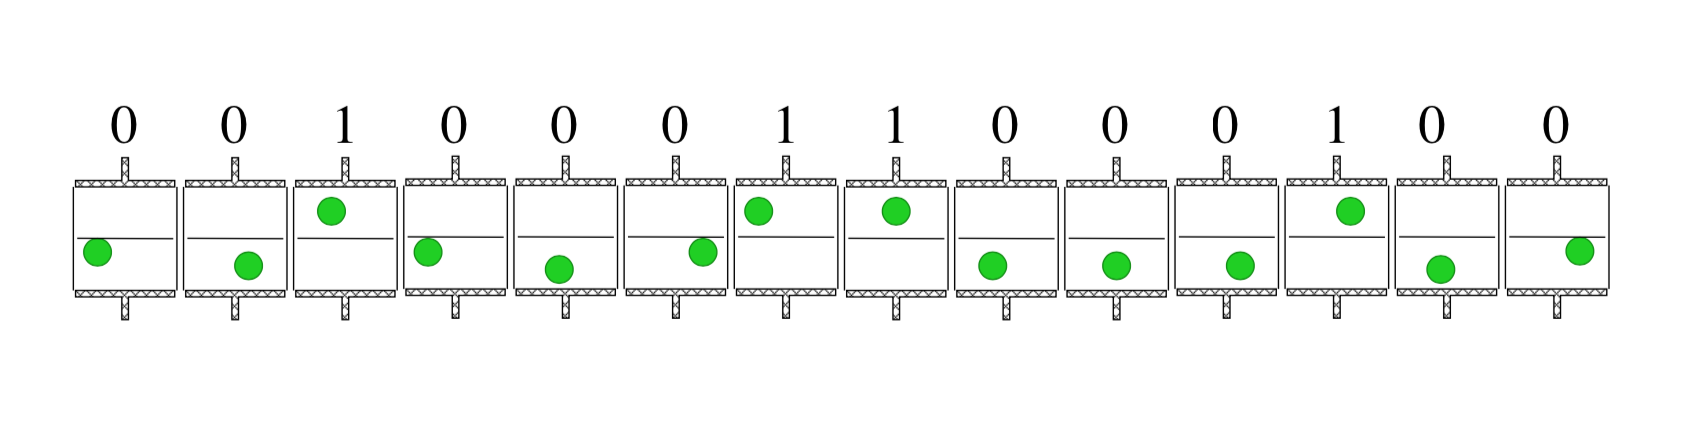
\includegraphics[width=0.4\linewidth]{Final_Fig1}
\caption{Minimalist digital memory tape.\label{fig:tape}}
\end{figure}

\begin{figure}[p]
\centering
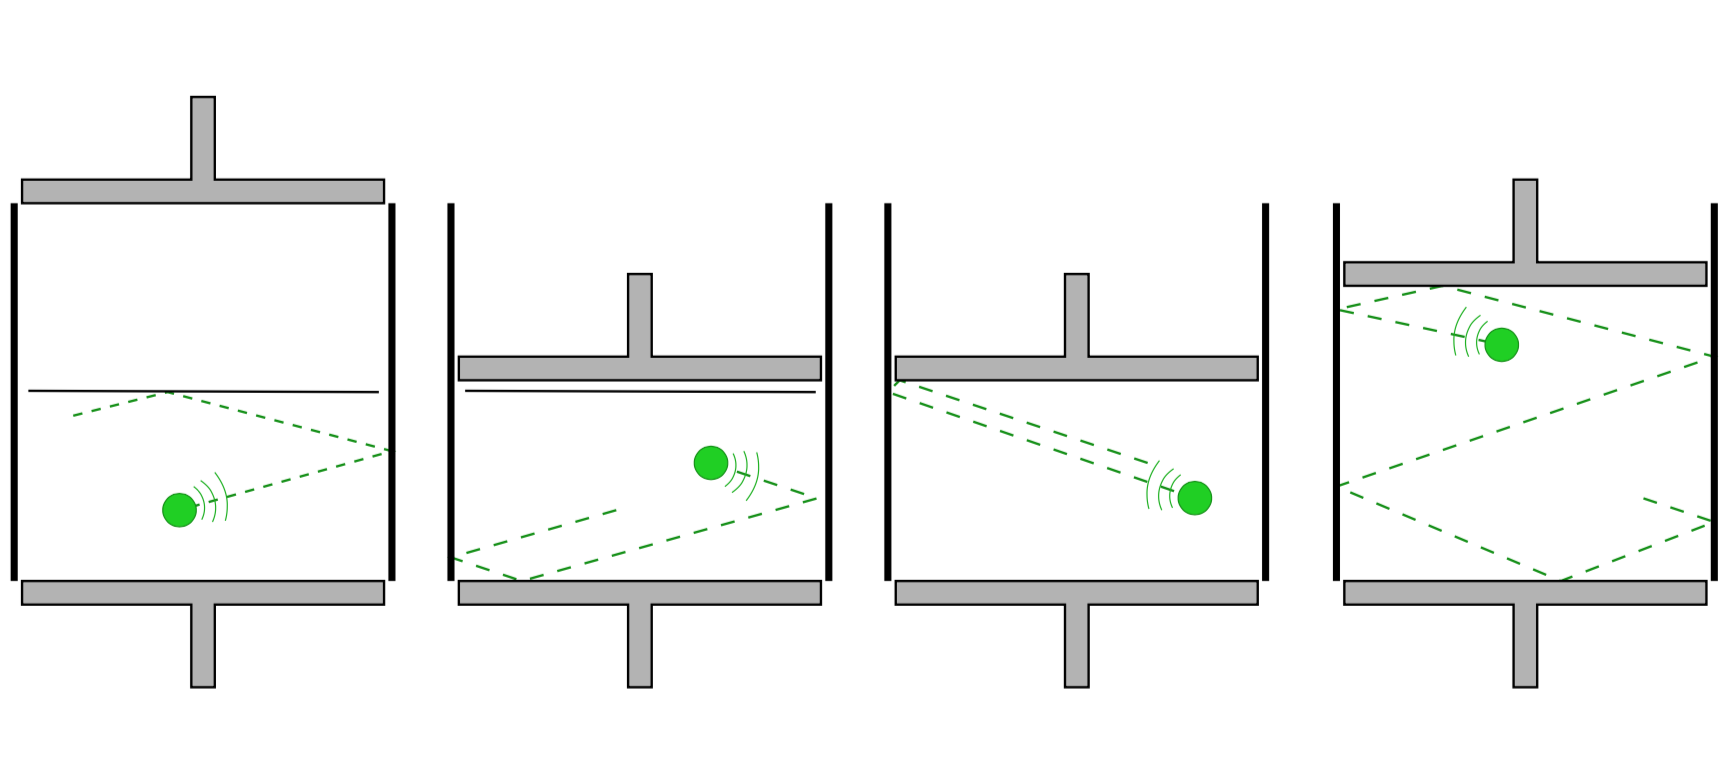
\includegraphics[width=0.4\linewidth]{Final_Fig2}
\caption{Expanding piston.\label{fig:piston}}
\end{figure}

\begin{figure}[p]
\centering
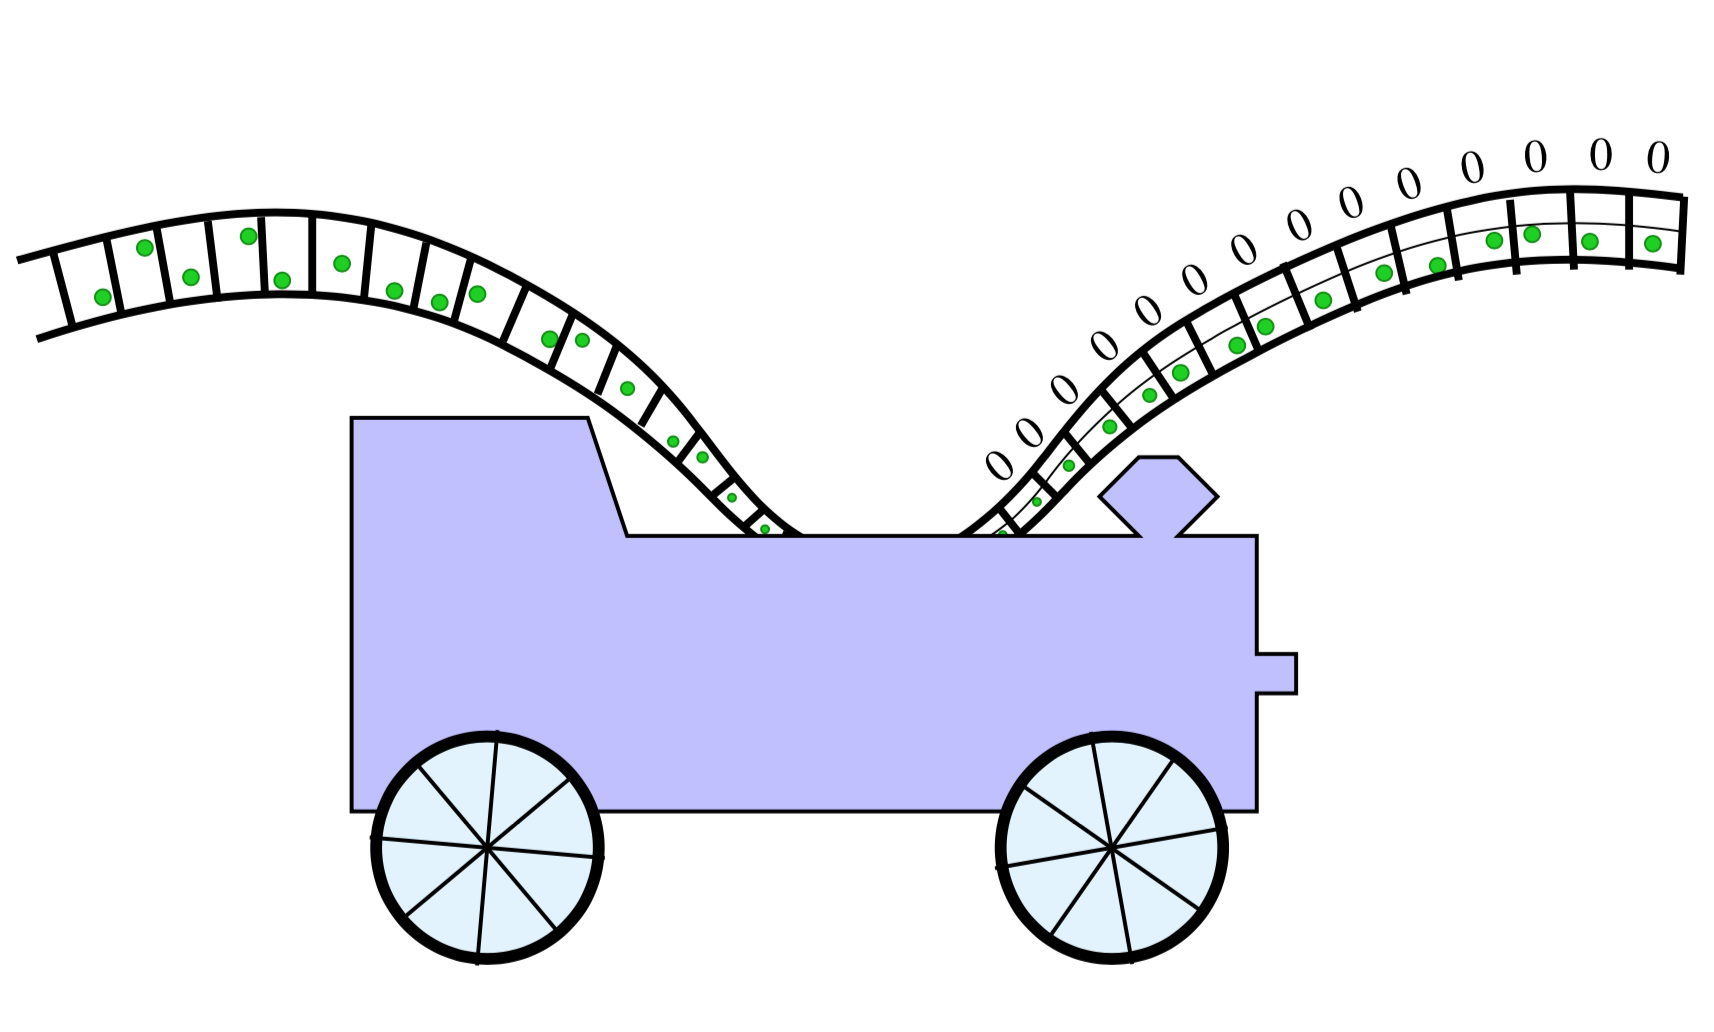
\includegraphics[width=0.4\linewidth]{Final_Fig3}
\caption{Information-burning engine.\label{fig:engine}}
\end{figure}

\begin{figure}[p]
\centering
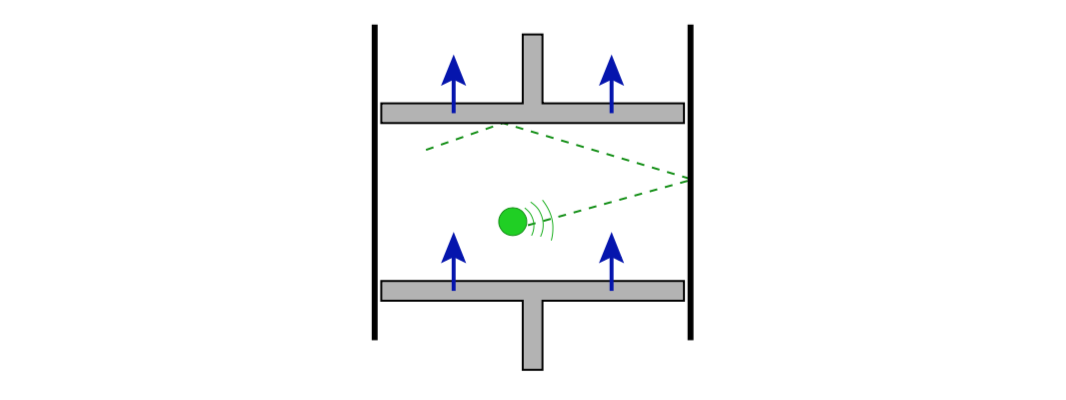
\includegraphics[width=0.4\linewidth]{Final_Fig4}
\caption{Pistons resetting a \textit{known} bit for free.\label{fig:zero}}
\end{figure}


Is there a minimum energy cost for taking a measurement? Let's try to find out. We start by addressing the connection between information entropy and thermodynamic entropy. Can we burn information as fuel?

Consider a really frugal digital memory tape, with one atom used to store each bit (fig~\ref{fig:tape}). The tape is a series of boxes, with each box containing one ideal gas atom. The box is split into two equal pieces by a removable central partition. If the atom is in the top half of the box, the tape reads one; else the tape reads zero. The side walls are frictionless pistons that may be used to push the atom around.

\emph{If} we know the atom position in the $n$th box, we can move the other side wall in, remove the partition, and gradually retract the piston to its original position (fig~\ref{fig:piston})--destroying our information about where the atom is, but extracting useful work.

\begin{question}
\textbf{(a)~Burning the information.} Assuming the gas expands at a constant temperature $T$, how much work $\int P\d{V}$ is done by the atom as the piston retracts?
\end{question}

\begin{solution}
This is an isothermal process; $T$ and $N$ are constant. Work in thermodynamic processes is given by $\int P\d{V}$, where $P = Nk_BT/V$. Before the piston retracts, $P_iV_i$ is equal to $Nk_BT$. We make this substitution in the integral. Finally we integrate to find the magnitude of the result. The final answer is \emph{negative}; work is being done \emph{by} the environment \emph{on} the atom and gas.
\begin{align}
\begin{aligned}
W& = - \int_{V_i}^{V_f} P \d{V}
= - P_iV_i \int_{V_i}^{V_f} \frac{\d{V}}{V}
\\
& = \boxed{P_iV_i \log \! \Bigg[ \frac{V_i}{V_f} \Bigg]}\label{eq:work}
\end{aligned}
\end{align}
\end{solution}

\newpage
\begin{question}
\textbf{(b)~Rewriting a bit.} Give a sequence of particle insertion, partition removal, and adiabatic side-wall motions that will reversibly convert a bit zero into a bit one, with no net work done on the system.
\end{question}

\begin{solution}
~
\\
\begin{enumerate}
\item Place the atom into the bottom half of the partitioned box. Our bit is now in state zero.

\item Adiabatically snap the top piston down to the position of the partition. Atom still bit zero. There is no time for heat transfer; entropy gain zero. This motion costs us work $W_1$ equal to what we calculated in part \textbf{(a)} (eq.~\ref{eq:work}).

\item Remove the partition from underneath the top piston and place it just above the bottom piston. The atom is now in the ``top'' part of the box (bit one).

\item Adiabatically snap the bottom piston down the same distance the top piston traveled; the volume of the box is now back to the initial value. The atom is in bit one state. This work done by the atom $W_2$ is equal to $-W_1$, thus we have successfully changed to atom from bit zero to bit one with zero net work done on the system.
\end{enumerate}
\end{solution}

\begin{question}
\textbf{(c)~Forgetting a bit.} Suppose the atom location in the $n$th box is initially known. What is the change in entropy, if the partition is removed and the available volume doubles? Give both the thermodynamic entropy and the information entropy
\end{question}

\begin{solution}
\textit{Thermodynamic entropy.} If we define thermodynamic entropy change to be the ratio of heat flow to temperature, we can argue $\Delta S_\text{thermo} = 0$ if we double the volume by adiabatically drawing the pistons back. In addition, it is difficult to define temperature for a single atom. However, we can still think of $\Delta S_\text{thermo}$ as entropy change of mixing.

We can write down the entropy of mixing as
\begin{align}
S& = k_B \log \Omega \label{eq:S},
\end{align}
where $\Omega$ is the configurational energy-shell volume. For $N$ atoms in a box, the number of configurations in a volume $V$ is given by $V^N/N!$. Thus for our atom in a box, $\Omega_i = V$ and $\Omega_f = 2\Omega_i$
\begin{align}
\Aboxed{\Delta S_\text{thermo} & = S_f - S_i = k_B \log \frac{\Omega_f}{\Omega_i} = k_B \log 2} \label{eq:DSthermo}
\end{align}

\textit{Information entropy.} We can write down information entropy generally as
\begin{align}
S_\text{info} & = - k_S \sum_k p_k \log p_k = - \sum_k p_k \log_2 p_k\label{eq:Sinfo},
\end{align}
where $p_k$ is the probability of each possible state $k$ of a bit. Before the volume is doubled, we already know the position of the atom in the box. Suppose we know it is in a bit zero state. The initial probability of the atom being in bit zero state is one; probability of bit one state is zero. Once we remove the partition and double the volume, we lose information about the atom's state. Each state becomes equally probable. We use this change in probabilities to write down $\Delta S_\text{info}$.\footnote{eqs.~\eqref{eq:DSthermo} \& \eqref{eq:DSinfo} differ by nothing more than a normalization factor. We write thermodynamic entropy in units of energy per temperature, hence the Boltzmann factor $k_B$. When speaking about the entropy of bits, it makes more sense to present our results in base 2.}
\begin{align}
S_i &= -k_S \cdot(1) \cdot \log 1 = 0
\\
S_f &= -k_S \cdot(2) \cdot \frac{1}{2} \log \frac{1}{2} = \log_2{2}
\\
\Aboxed{
\Delta S_\text{info}  &= S_f - S_i = k_S \log{2} = 1}\label{eq:DSinfo}
\end{align}
\end{solution}

\begin{question}
\textbf{(d)~Demonic states.} What prevents a Maxwellian demon from using an atom in an unknown state to extract work? The demon must first measure which side of the box the atom is on; this measurement needs no energy expenditure. (i) After the bit has been burned (see fig~\ref{fig:engine}), is the demon in a known state?\footnote{The demon can be thought of as a two-state system (e.g.~another partitioned box). If the demon starts in a known state, one can copy the state of the box into the demon with no cost in entropy or energy, by adiabatically turning on an appropriate coupling. The demon has now measured the atom position, and can extract work from the pistons.}
(ii) What is its entropy? (iii) How much energy would it take to return the demon to its original state, at temperature T? (iv) Is the second law violated?
\end{question}

\begin{solution}
~\\
\begin{enumerate}
\item[(i)] \boxed{\text{Yes,}} after the bit has been burned, the demon is in a known state. The information from the bit has been copied to the demon prior to the bit's burning-for-work.

\item[(ii)] Burning the bit, however, costs us entropy. Initially the bit was in a low entropy state. The cost of ``forgetting a bit'' is given by $\boxed{k_B \log{2}}$ (see eqs.~\ref{eq:DSthermo} \& \ref{eq:DSinfo}).

\item[(iii)] It would take \boxed{0} energy to return the demon to its original state, at temperature $T$. Its original state was a random state. We can wipe a bit by removing the partition and moving both pistons adiabatically in the same direction for a certain distance (see fig~\ref{fig:zero}).

\item[(iv)] The Second Law of Thermodynamics states that the entropy of a closed system never decreases over time. This law is \boxed{\text{not violated.}} We can extract an unlimited amount of work with a demon by copying information from one bath to another. However, whenever we take energy from a bath, we have to pay for it with entropy. This is a fundamental truth about the Universe.
\end{enumerate}
\end{solution}


























%%%%%%%%%%%%%%%%%%%%%%%%%%%%%%%%%%
%% ENTROPY INCREASES: DIFFUSION %%
%%%%%%%%%%%%%%%%%%%%%%%%%%%%%%%%%%
\newpage
\section{Entropy increases: diffusion}

Entropy technically does not increase for a closed system. However, in most of the coarse-grained theories, entropy does increase; when we integrate out degrees of freedom, we provide a means for the information about the initial conditions to be destroyed.

Let $\rho(x,t)$ obey the one-dimensional diffusion equation $\pdv*{\rho}{t} = D\pdv*[2]{p}{x}$. Assume that the density $\rho$ and all its gradients die away rapidly at $x = \pm \infty$.\footnote{Also, assume $\pdv*[n]{\rho}{x} \log{\rho}$ goes to zero at $x = \pm \infty$, even though $\log{\rho}$ goes to $-\infty$.}

\begin{question}
Derive a formula for the time derivative of the entropy $S = -k_B \int \rho(x)\log{\rho(x)} \d{x}$ and show that it is strictly increasing in time.
\end{question}



\begin{solution}
We start by taking the time derivative of the definition of entropy.
\begin{align}
S &= -k_B \int_{\text{all space}} \rho \log{\rho} \d{x}
\\
\pdv{S}{t} &= -k_B \int \dot{\rho} \log{\rho} + \dot{\rho} \d{x}
\end{align}
Since $\rho$ obeys the diffusion equation, we can make the following substitution.
\begin{align}
\dot{S} &= -Dk_b \int \rho'' \log{\rho} + \rho'' \d{x}
\\
\dot{S} &= -Dk_B \bigg[\cancelto{0}{\rho'\eval_{-\infty}^{\infty}} + \int  \rho'' \log{\rho} \d{x}\bigg]
\\
\dot{S} &= -Dk_B \int \rho'' \log{\rho} \d{x}
\end{align}
The $\rho''$ term dies out when integrated over all space because we are assuming the probability density and all its gradients die out at the boundaries.

Next, we will try to get the remaining integrand into a form that is always positive. We will use the \textsc{di} method for integration by parts.

\begin{center}
\begin{tabular}{lrl}
		& 	D		& 	I
\\
+		&		$\log{\rho}$		&		$\rho''$
\\
-		&		$\frac{1}{\rho}\rho'$		&		$\rho'$
\end{tabular}
\end{center}
\begin{align}
\dot{S} &= -Dk_B \int \rho'' \log{\rho} \d{x} = -Dk_B \bigg[ \cancelto{0}{\rho'\log{\rho}\eval_{-\infty}^{\infty}} - \int \frac{(\rho')^2}{\rho} \d{x}    \bigg]
\end{align}
After integrating by parts, our first term dies again because of our initial assumption regarding the probability density (see footnote). We are left with the following integrand.
\begin{equation}
\dot{S} = Dk_B \int \frac{(\rho')^2}{\rho} \d{x}\label{eq:4.0}
\end{equation}
We cannot evaluate this integral, but we don't need to. First, consider the $1/\rho$ term. $\rho(x,t) \in [0,1]$ is a probability density, it cannot physically be negative. Next, consider the $(\rho')^2$ term. The square of any number is always positive. So although we do not know what $\rho'$ looks like, we only care about its square. Therefore, we know that the integrand in eq.~\eqref{eq:4.0} will always be positive for all values of $x$ that we are integrating over.

We can confidently say that the time derivative of entropy is always increasing.
\begin{align}
\Aboxed{
\pdv{S}{t} &\geq 0}
\end{align}
\end{solution}































%%%%%%%%%%%%%%%%%%%%%%%%%%%%%%%%%%%%%%%%%%%%%%%
%% PHASE SPACE UNITS AND THE ZERO OF ENTROPY %%
%%%%%%%%%%%%%%%%%%%%%%%%%%%%%%%%%%%%%%%%%%%%%%%
\newpage
\section{Phase-space units and the zero of entropy}

In classical mechanics, entropy goes to minus infinity at the temperature is lowered to zero. In quantum mechnics the entropy per particle goes to zero, because states are quantized and the ground state is the only one populated.

The classical phase-space shell volume $\Omega(E)\var E$ has units of ([momentum]$\cdot$[distance])$^{3N}$. We can make it unitless with Planck's constant $h^{3N}$; if we measure phase-space volume in units of $h$ per dimension, $\Omega(E)\var E$ will be dimensionless. Of course, the correct dimension could be a constant times $h$, like $\hbar \ldots$

\begin{question}
\textbf{(a)}~\textbf{Arbitrary zero of the classical entropy.} Show that the width of the energy shell $\var E$ in the definition of $\Omega(E)$ does not change the microcanonical entropy per particle
\begin{equation}
S/N = k_B\log{\Omega(E})/N\label{eq:5.0}
\end{equation}
in a large system. Show that the choice of units in phase space does change the classical entropy per particle.
\end{question}

\begin{solution}
The definition of classical phase-space is
\begin{equation}
\Omega(E) = \frac{1}{\var E}\int_{H < E < H+ \var E } \d{\mathbb{P}} \d{\mathbb{Q}}
\end{equation}
For our ensemble, we assume particles are non-interacting, so we do not have to integrate over configurations $\mathbb{Q}$. The integral over momenta $\mathbb{P}$ is equal to the difference in volumes of $3N$ dimensional spheres of radii $\sqrt{2m(E + \delta E)}$ and $\sqrt{2mE}$. When we take the logarithm of the different of phase-space volumes for each sphere, we find that the exponents are eliminated thanks to the nifty properties of logarithms, and the $\var E$'s cancel out.
\begin{align}
\Omega(E) &= \frac{1}{\var E} \frac{\pi^{3N/2}}{(3N/2)!} \Bigg[ (2m(E + \delta E))^{3N/2} -  (2mE)^{3N/2}\Bigg]
\\
S &= k_B \log(\frac{1}{\var E} \frac{\pi^{3N/2}}{(3N/2)!} \Bigg[ (2m(E + \delta E))^{3N/2} -  (2mE)^{3N/2}\Bigg])
\\
&= k_B \Bigg[ \log{\frac{\pi^{3N/2}}{(3N/2)!}} + 3N/2\log( 2m(E + \var E) - 2mE) - \log(\var E)   \Bigg]
\\
S/N &= k_B \Bigg[ \frac{1}{N} \log{\frac{\pi^{3N/2}}{(3N/2)!}} + 3/2\log{2m} + 3/2\log{\var E} -\log{\var E}    \Bigg]
\end{align}
The value of $1/2 \log{\var E}$ is very small, so in the end we have shown that $S/N$ is independent of $\var E$.

However, if we chose the normalize our phase-space volume with $h^{3N}$ or $\hbar^{3N}$, we would get a different result. Therefore, choice of units in phase-space does matter.
\end{solution}



\begin{question}
\textbf{(b)}~\textbf{Phase-space density of states for a  particle in a one-dimensional box.} Show, or note, that the quantum momentum-space density of states for a free quantum particle in a one-dimensional box of length $L$ with periodic boundary conditions is $L/h$. Draw a picture of the classical phase space of this box $(p,x)$, and draw a rectangle of length $L$ for each quantum eigenstate. Is the phase-space area per eigenstate equal to $h$, as assumed?
\end{question}

\begin{solution}
In quantum mechanics, energy states are quantized. The energy eigenstates for a 1-$D$ particle in a box are $E_n = \frac{n^2 h^2}{8m^2 L^2}$. Therefore, the momentum per eigenstate are $p_n = \frac{nL}{2L}$. Taking into account the periodic boundary conditions (accounts for the factor of 2), we find that the phase space volume is indeed $L/h$.
\begin{figure}[h!]
\centering
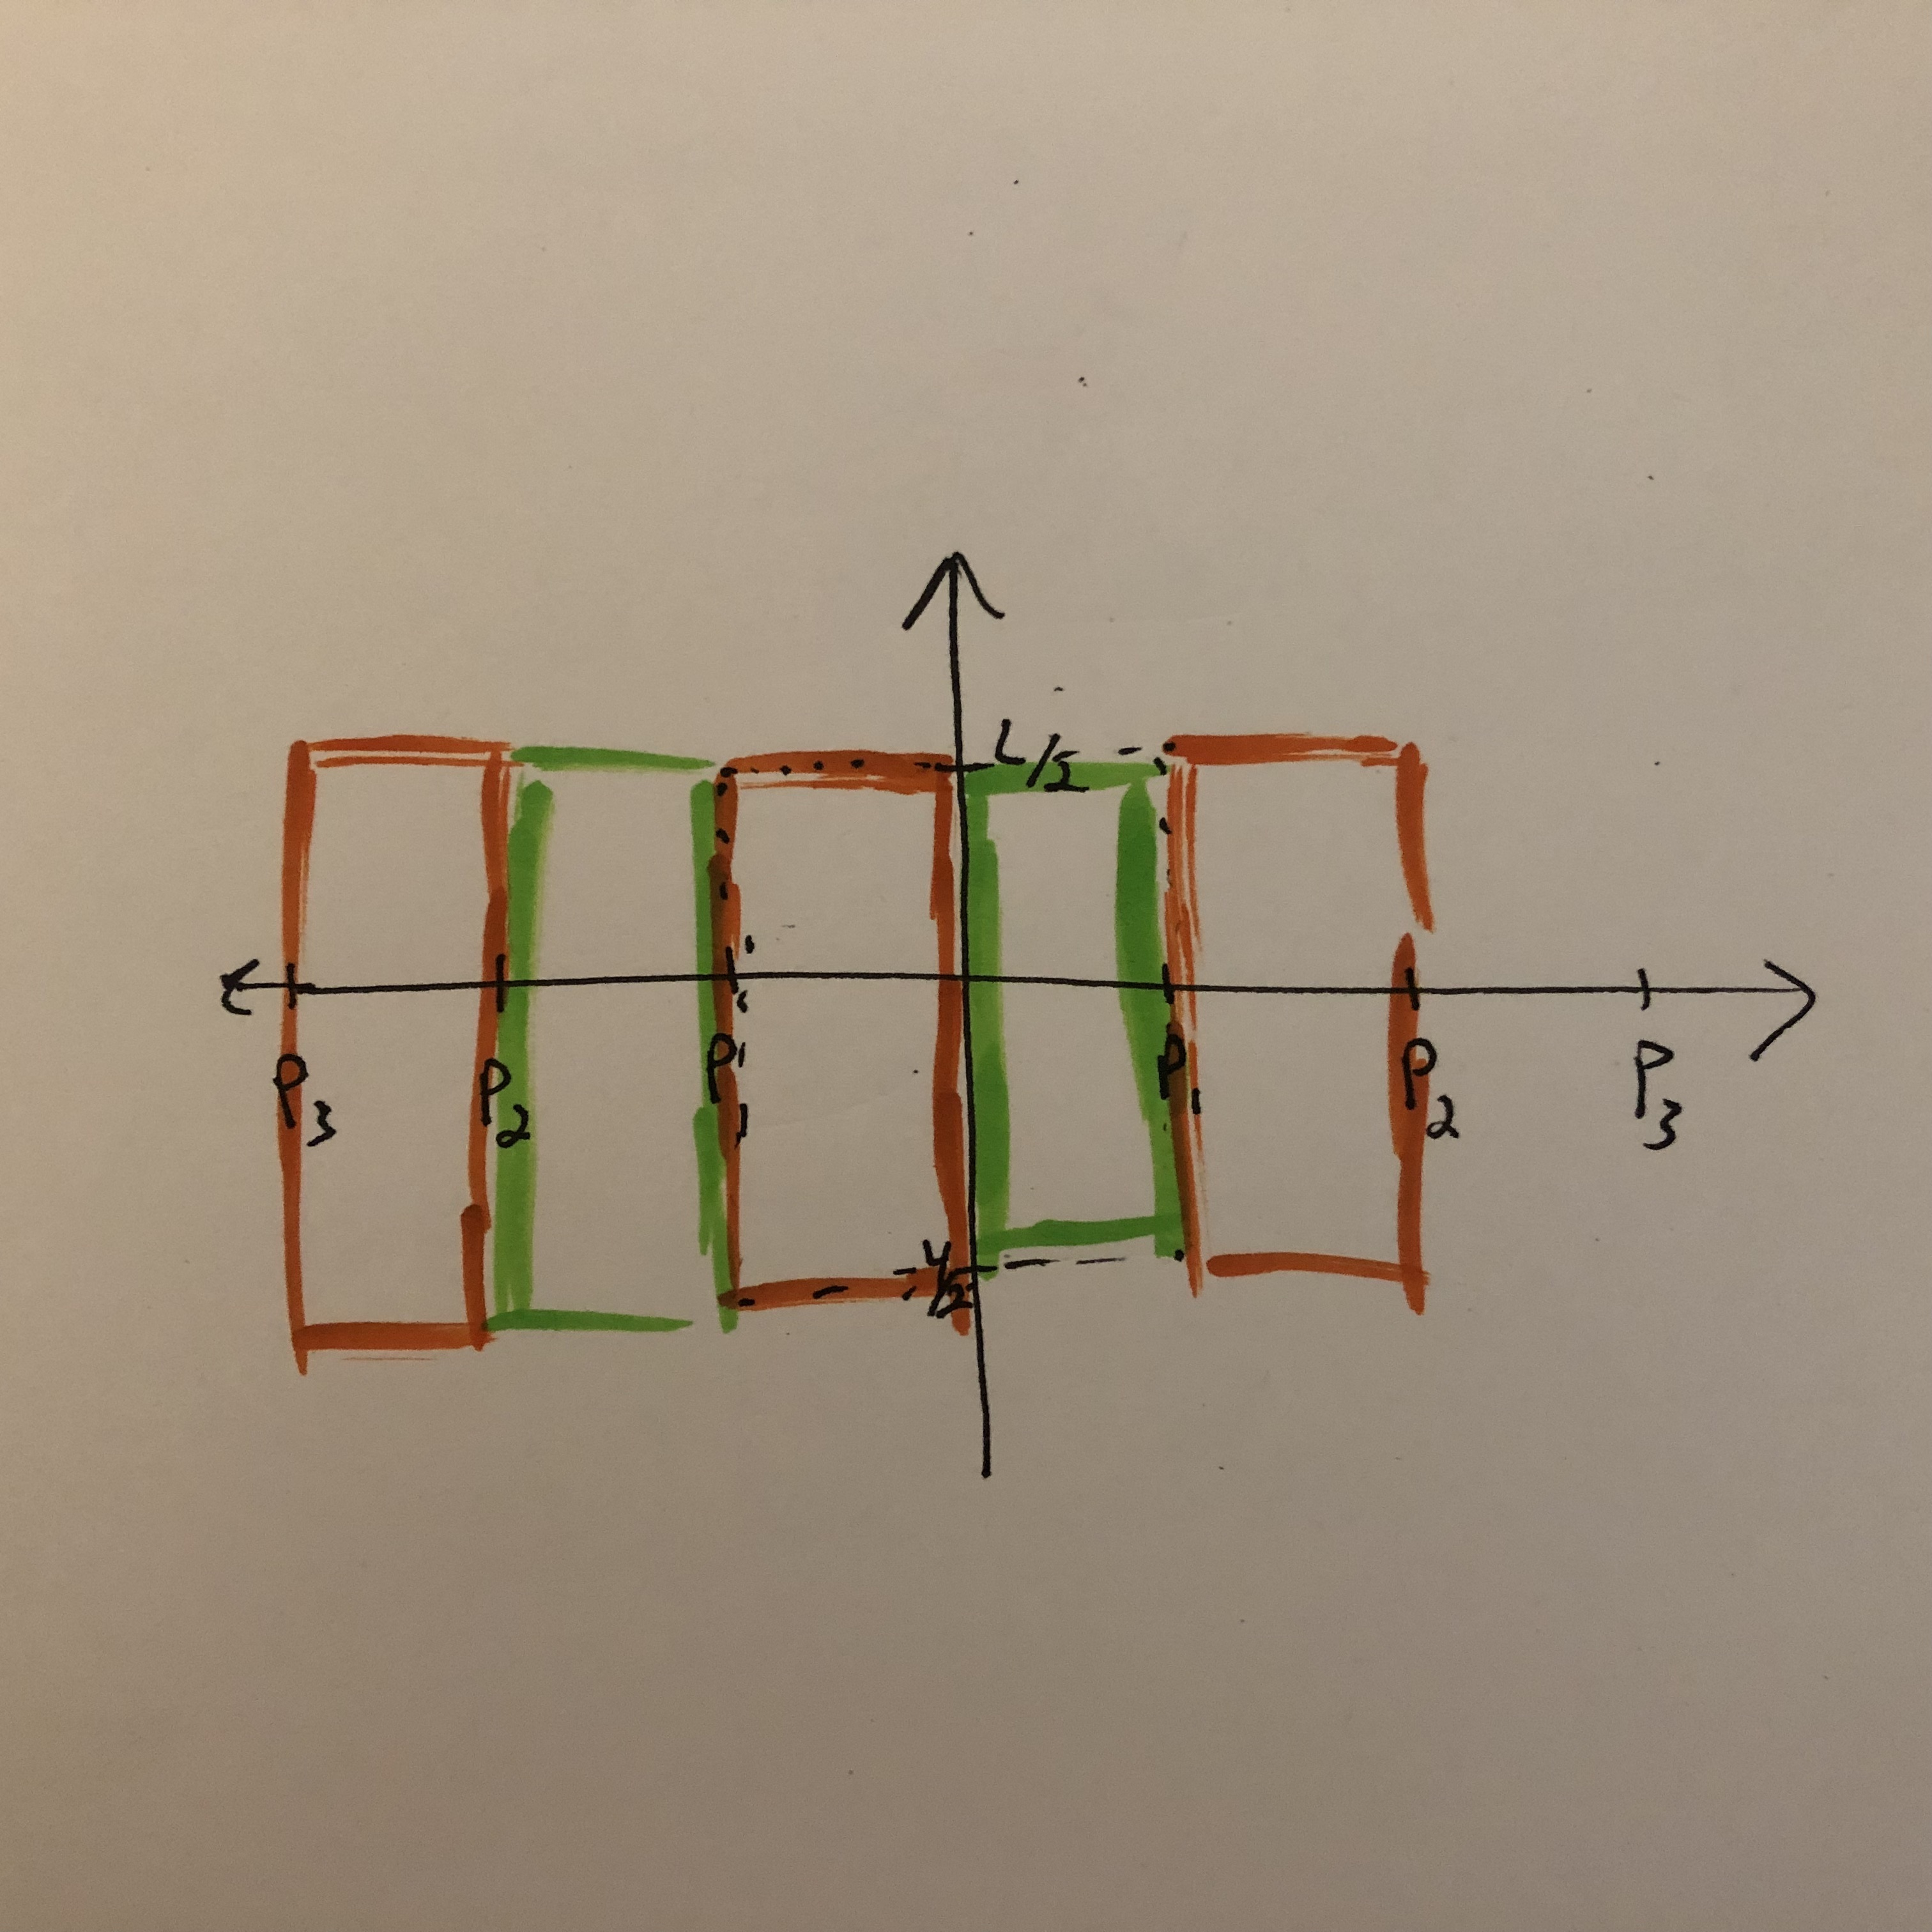
\includegraphics[width=.3\linewidth]{Final_Fig5}
\caption{Phase-space volume of a 1-D particle in a box.}
\end{figure}
The phase-space volume per eigenstate is indeed equal to $h$.
\end{solution}


\begin{question}
\textbf{(c)}~\textbf{Phase-space density of states for $N$ particles in a box.} Show that the density of states for $N$ free particles in a cubical box of volume $V$ with periodic boundary conditions is $V^N/h^{3N}$, and hence that the phase-space volume per state is $h^{3N}$.
\end{question}

\begin{solution}
The energy eigenstates are given by $E_{nx,ny,nz} = \frac{\hbar^2 \vb{k}^2}{2m}$ and we find that each 3D wave vector is given by
$k = \frac{n_x \pi}{L} + \frac{n_y \pi}{L} + \frac{n_z \pi}{L}$. Therefore the phase space volume for one particle is given by $V/h^3$. If we have $N$ particles in a box, each occupies a respective volume, so we take our answer and raise it to the power of $N$. The phase-space volume then turns out to be $V^N/h^{3N}$, and the volume per state is $h^{3N}$.
\end{solution}


\begin{question}
\textbf{(d)}~\textbf{Phase-space density of states for a harmonic oscillator.} Consider a harmonic oscillator with Hamiltonian $\mathcal{H} = p^2/2m + 1/2 mw^2q^2$. Draw a picture of the energy surface with energy $E$, and find the volume of phase space enclosed. What is the volume per energy state?
\end{question}

\begin{solution}
For a fixed energy, the phase-space volume turns out to be elliptical. The volume (or rather area) is given by $\pi p x$.

\begin{figure}[h!]
	\centering
	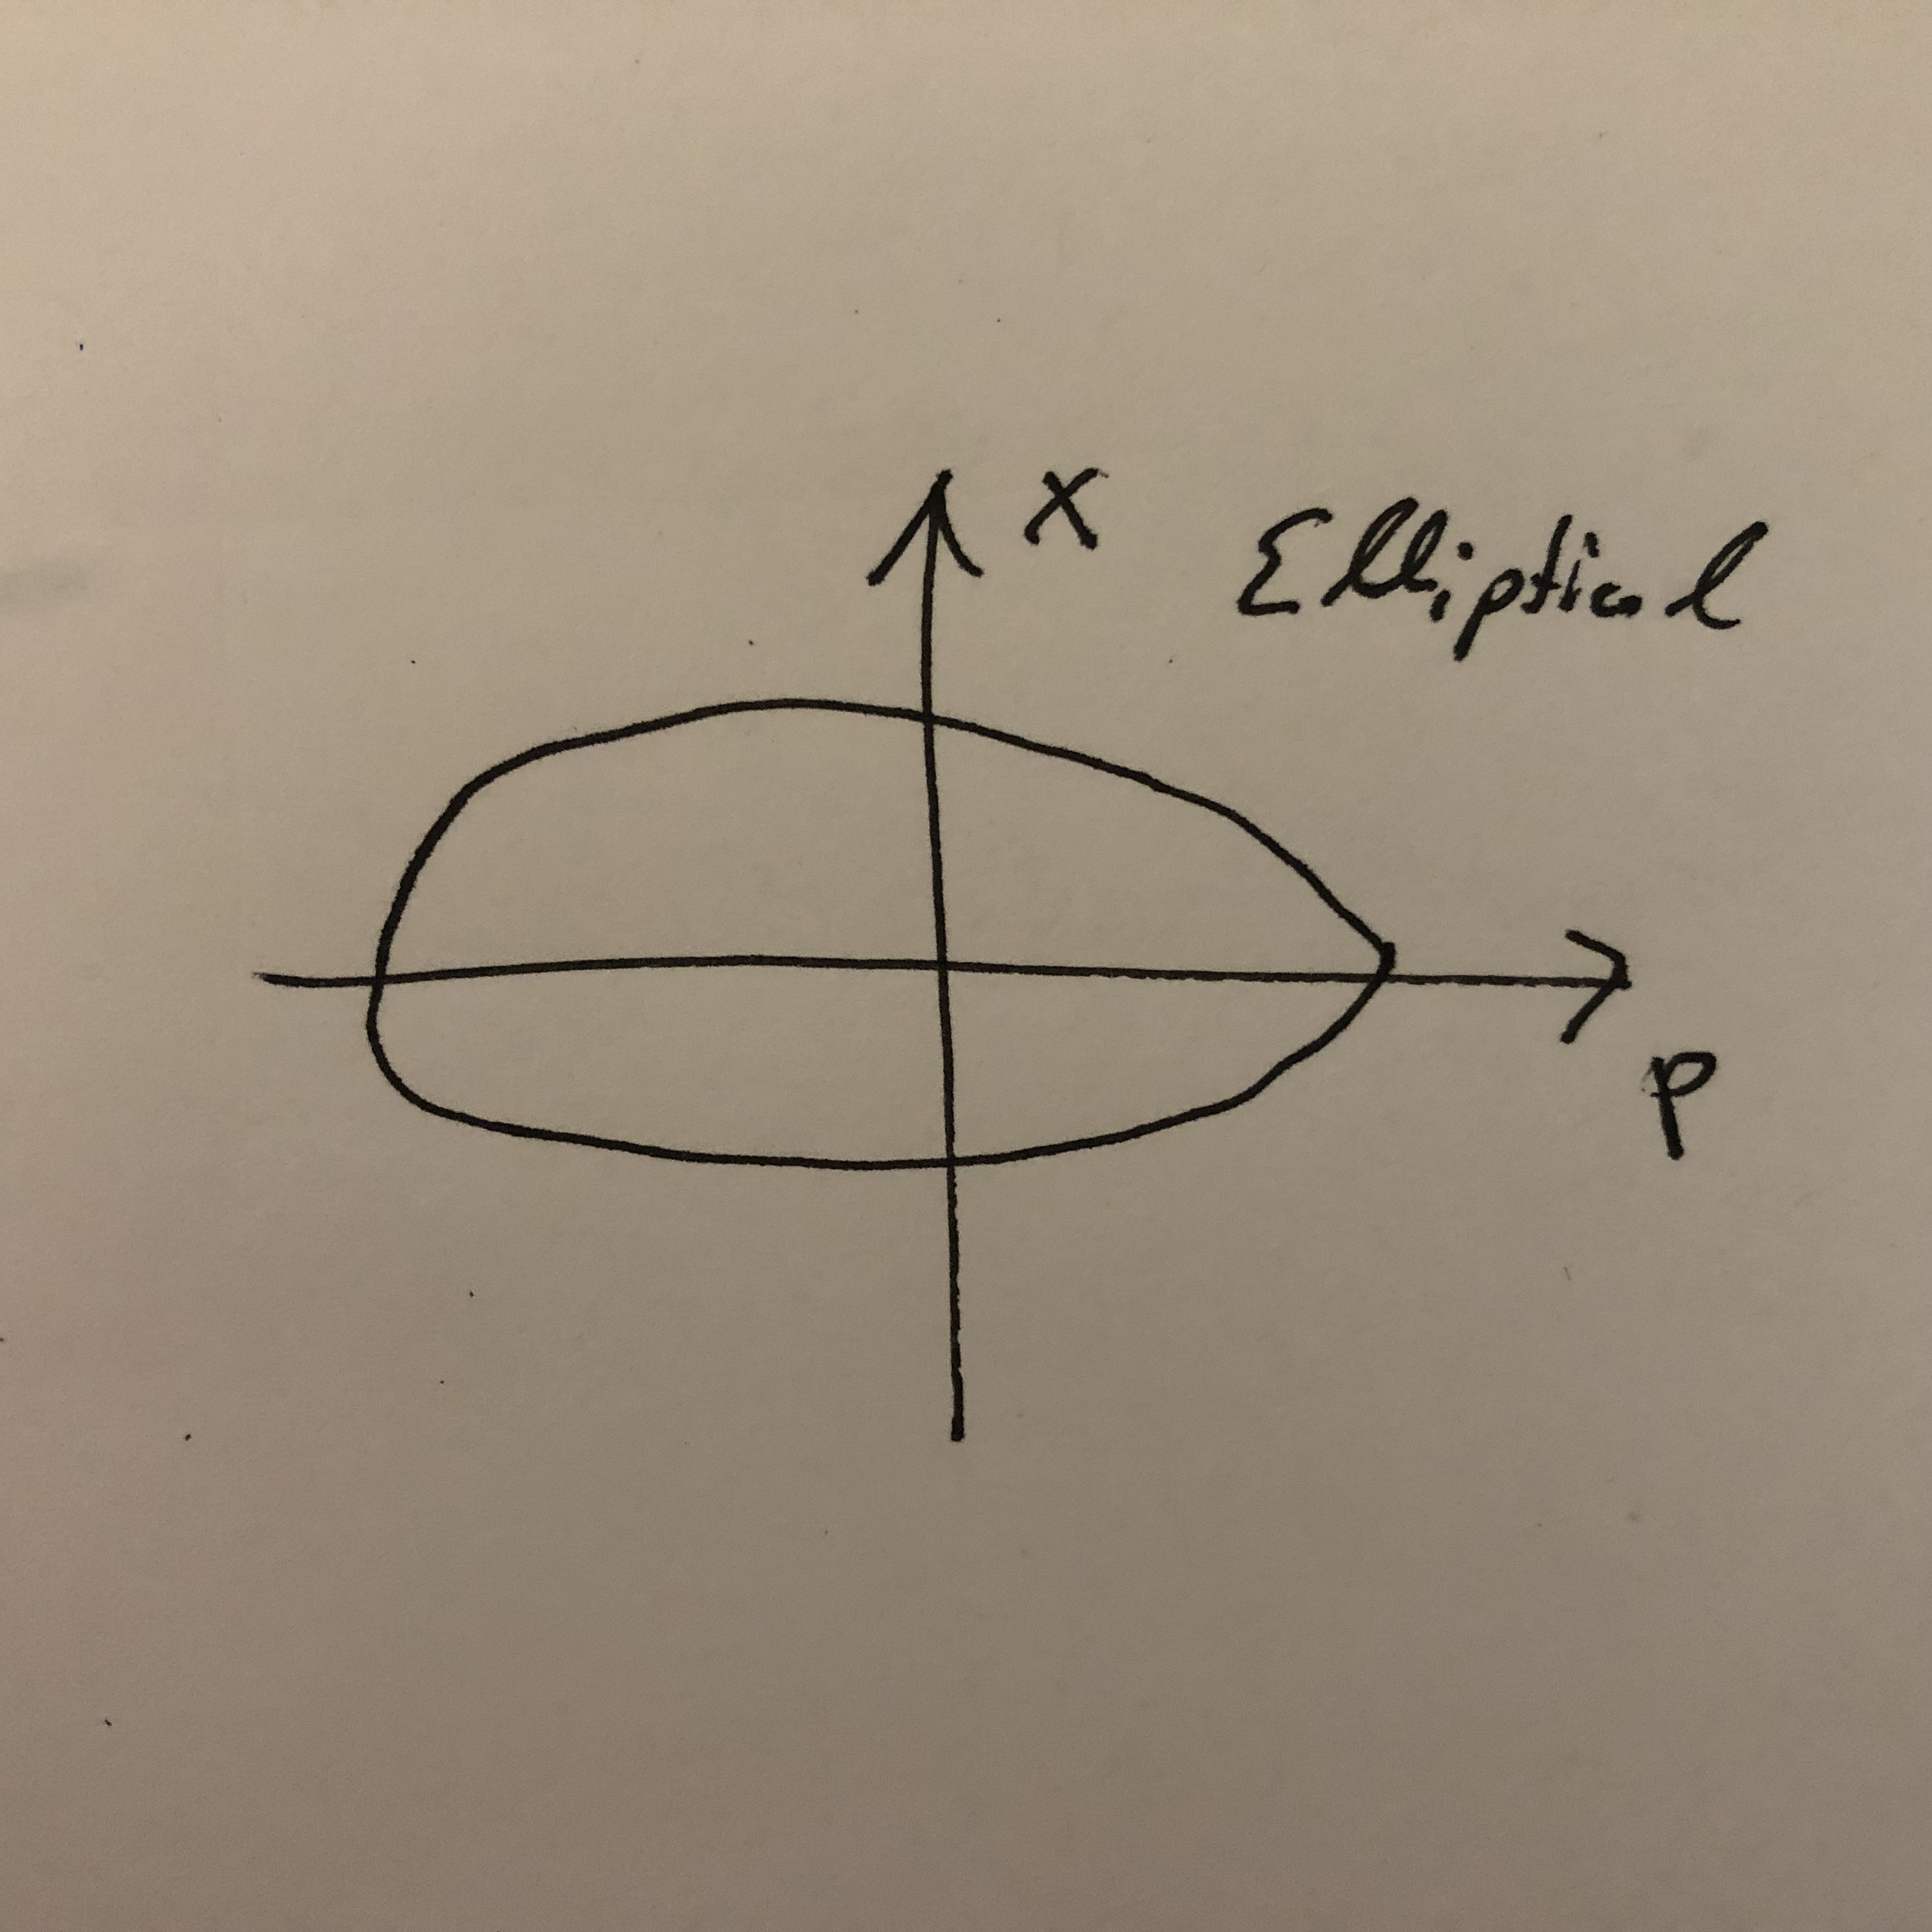
\includegraphics[width=.3\linewidth]{Final_Fig6}
	\caption{Phase-space volume of a quantum harmonic oscillator with energy $E$.}
\end{figure}

\end{solution}























%%%%%%%%%%%%%%%%%%%%%%%
%% AN UNLIKELY EVENT %%
%%%%%%%%%%%%%%%%%%%%%%%
\newpage
\section{An unlikely event}

On June 12, 2019 at 6:59 pm, you are exiting the elevator, walking toward \textsc{ms\&e} to hand in your final take home exam for Physics 133. Just a few moments before 6:59 pm, a small meteor falls from the sky and crashes into a physics textbook on the desk of a philosopher trying to understand the meaning of entropy. The meteor is burning at such a high temperature that it instantly incinerates the book and continues burning through floor after floor of the building until coming to rest near a water line adjacent to a 50 year-old water fountain. The pipe becomes super heated, compressing the water in the plumbing and causing a catastrophic failure of the building’s pipes. The compression shock shakes the foundation of the building and, just as you exit the elevator, a micro-earthquake rumbles across the entire campus. Your exam slips from your hands and falls like an autumn leaf right between the crack that separates the elevator from the third floor's surface. The exam can't be recovered. Assume that the observation of this event is extremely unlikely. How much information is contained in such an event?

\begin{question}
\textbf{(a)} From Shannon, we know that the entropy is in fact a measure of \textit{information}. Suppose that any event, including that described above, occurs with probability $p$. We can associate with the observation of this event a function that quantifies the amount of information, call it $I(p)$. Find the functional form of $I(p)$ such that the following conditions are met:
\begin{enumerate}
\item Information is \textit{non-negative}.
\item If two events occur independently so that their joint probability is the product of event 1 and event 2, then their information is \textit{additive}.
\item Information is a continuous function of the probability $p$.
\item There is \textit{no information} content to an event that is always observed.
\end{enumerate}
\end{question}

\begin{solution}
We need a function that satisfies the following four criteria.
\begin{enumerate}
\item Information is non-negative.
\begin{align}
I(p) & \geq 0
\end{align}

\item For two independent events $i$ and $j$ where the joint probability that they both occur is $p_i \cdot p_j$, the total information of the events is given by $I(p_i) + I(p_j)$.
\begin{align}
I(p_i) + I(p_j) & = I(p_i + p_j)
\end{align}

\item Information is a continuous function of the probability $p$. A function $I$ is continuous if and only if the limit
\begin{equation}
\lim_{p \to a} I(p) = I(a)
\end{equation}
exists.

\item If an event $i$ is always observed, that event contains no information such that
\begin{align}
\text{for an event $i$, if $p_i = 1$, then}\  I(p_i)& = 0.
\end{align}
\end{enumerate}
A simple function that has these four properties is the logarithm function.\footnote{Proofs left as an exercise for the reader. Or see \url{https://en.wikipedia.org/wiki/Logarithm}.} Let
\begin{align}
\Aboxed{I(p) & = - \log{p} = \log{\frac{1}{p}}}\label{eq:info}
\end{align}
where $p \in [0,1]$ is the probability of a given event occurring.
\end{solution}

\begin{question}
\textbf{(b)} Find the value of $I(p)$ for the event described above (i.e.~the probability of observing such an event approaches zero). How much information is contained in an event as unlikely as this one?
\end{question}

\begin{solution}
The chances of such an event happening are \textbf{unlikely}. Let the probability of the unlikely event occurring go to zero. The amount of information contained in the event is given by
\begin{equation}
\boxed{I(p) = \lim_{p \to 0}  \log\frac{1}{p} = \infty.}
\end{equation}
The amount of information contained in this event is infinite.
\end{solution}

\end{document}
